%  Typ dokumentu - článek, prezentace aj.
\documentclass[english]{article}

%  Nastaví vstupní a výstupní kódování znaků (encoding) a lokalizace
\usepackage[T1]{fontenc}
\usepackage[utf8]{inputenc}
\usepackage[english,czech]{babel}
\usepackage{icomma}
\usepackage{lmodern}

%  Formát papíru a odsazení od jeho okrajů
\usepackage[letterpaper]{geometry}
\geometry{verbose,tmargin=1.5cm,bmargin=2cm,lmargin=2cm,rmargin=2cm}

%  Umožňuje pracovat s grafikou
\usepackage{graphicx}

%  Automaticky odsadí i první paragraf v každé sekci
\usepackage{indentfirst}

%  Umožňuje rozdělovat obsah na více sloupců
\usepackage{multicol}

%  Umožňuje používat hypertextové odkazy, nastavuje jejich barvu a
%  vlastnosti
\usepackage[unicode]{hyperref}
\hypersetup{
colorlinks=true, citecolor=blue, filecolor=blue, linkcolor=blue,
urlcolor=blue
}

%  Umožnění odstranění italiky u jednotek
\newcommand{\unit}[1]{\mathrm{#1}}

%  Formátování stránek, empty = odstraní číslování
% \pagestyle{empty}

%  Řádkování
\linespread{1.2}

%  Lepší zobrazování matematiky (rozšíření sum o \limits atd.)
\everymath{\displaystyle}

% Umožní psát přes \mathbb{N/R/Q/..} množiny čísel
\usepackage{amssymb}

%  Velikost fontu matematických výrazů v dokumentu lze pro danou
% základního fontu dokumentu upravit pomocí:
% \DeclareMathSizes{X}{Y}{Z}{U} kde:
% X je velikost fontu v dokumentu, pro kterou se matematika upraví
% Y je standartní velikost fontu matematiky
% Z je velikost fontu zmenšených (vnořených výrazů)
% U je velikost fontu ještě více zmenšených (vnořených výrazů).
\DeclareMathSizes{10}{10.5}{9}{9}

%  Nastaví autora, název, datum, skupinu měření apod. (můj vlastní
% příkaz, umožní znovu-použití v dokumentu)
\newcommand{\Author}{David Roesel}
\newcommand{\Coauthor}{Tereza Schönfeldová}
\newcommand{\Institute}{FJFI ČVUT v Praze}
\newcommand{\Subject}{FYZIKÁLNÍ PRAKTIKUM I}
\newcommand{\Group}{7}
\newcommand{\Circle}{ZS 5}
\newcommand{\Title}{Úloha \#8 \\Studium ultrazvukových vln.}
\newcommand{\Date}{11.10.2013}

% Začátek dokumentu - Formátování na výstup
\begin{document}

% Interní proměnné, možno zobrazovat u prezentací, používají se při
% generování pomocí \titlepage apod.
\author{\Author}
\title{\Title}
\date{\Date}

%  Lokalizace některých názvů do češtiny
\renewcommand{\figurename}{Obr.}
\renewcommand{\tablename}{Tab.}
\renewcommand{\refname}{Reference}

% --- Hlavička dokumentu -----------------------------------------------

\setlength{\parindent}{0cm}
\begin{multicols}{2}
\textbf{\Subject \\
        \Institute \\[0.1cm]
\large  \Title \\[0.5cm]
}
\begin{tabular}{rlrl}
\large Datum měření: & \Date & \large Skupina: & \Group \\
\large Jméno: & \Author & \large Kroužek:  & \Circle\\
\large Spolupracovala: & \Coauthor &\large Klasifikace:\\
\end{tabular}

\begin{flushright}

\includegraphics[scale=0.28]{../../_meta/fjfi_standart.pdf}
\hspace{0.2cm}
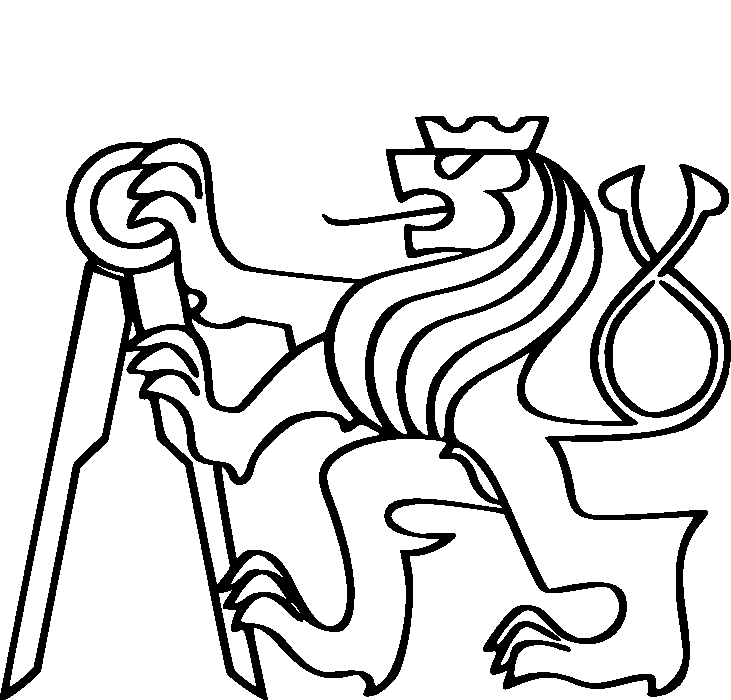
\includegraphics[scale=0.28]{../../_meta/cvut_standart.pdf}
\end{flushright}
\end{multicols}
\hrule
\vspace{0.5cm}

% ----------------------------------------------------------------------


% --- Tělo dokumentu ---------------------------------------------------

% Ocitovat markovu hlavičku
% Zeptat se na značky přístrojů

\setlength{\parindent}{0.5cm}

\section{Pracovní úkoly}
\begin{enumerate}
  \item Změřte velikost přijímaného signálu v závislosti na úhlu mezi přijímačem a kolmicí k odrazové ploše. Výsledky zpracujte tabulkově a graficky, a ověřte, zda-li platí zákon odrazu pro ultrazvukové vlny. Měření proveďte pro 3 různé úhly dopadu.
  \item Změřte rychlost zvuku ve vzduchu. Proveďte alespoň deset měření při různých vzdálenostech vysílače od přijímače a výsledky zpracujte statisticky. Porovnejte vás výsledek se vztahem \ref{eq:teorie_rychlost_zvuku}.
  \item Změřte alespoň pět vzdáleností odrazové plochy od vysílače/přijímače pomocí ultrazvukových vln (princip sonaru). Porovnejte vzdálenosti měřené sonarem a měřítkem. Použijte vámi experimentálně stanovenou rychlost zvuku z úkolu 2.
  \item Změřte Dopplerův jev pro dvě rychlosti $v$ vozíčku pro oba případy (přijímač klid nebo přijímač pohyb) a porovnejte výsledky s teoretickými výpočty. Měření proveďte pro každý případ - přijímač klid/pohyb - a pro každou rychlost minimálně pětkrát.
  \item Proměřte závislost intenzity zvukového signálu po průchodu zvukových vln soustavou štěrbin pro N (počet štěrbin) = 1,2,5. Výsledky zpracujte graficky a okomentujte v protokolu.
\end{enumerate}

\section{Vypracování}

\subsection{Použité přístroje}
Generátor 40kHz vln, zesilovač, 2 mikrofony, dvoukanálový digitální osciloskop, čítač Tesla, odrazová
kovová deska, laboratorní stojan, parabolický odražeč, difrakční mřížka s nastavitelným počtem štěrbin, elektrický
vozíček s nastavitelnou rychlostí pojezdu, pojezdová lavice s měřítkem (2 ks), svinovací metr (3m), papírový úhloměr, kabely, sada držáků pro mikrofony, mobilní telefon.

\subsection{Teoretický úvod}

	\subsubsection{Rychlost zvuku}
		Celou úlohu budeme pracovat s ultrazvukovými vlnami, které jsou definovány jako vlny nad 20 kHz. Rychlost zvuku $v_z$ záleží na fázové rychlosti zvukových vln. Tato fázová rychlost $v_f$ závisí na objemové pružnosti prostředí $K$ a na hustotě tohoto prostředí $\rho$. Za předpokladu, že se vzduch chová jako ideální plyn, je šíření zvuku v plynech adiabatický děj a pro rychlost zvuku ve vzduchu platí vztah
		
		\begin{equation}
			v_z = v_f = \sqrt{\frac{K}{\rho}} = \sqrt{\frac{\gamma p}{\rho}},
			\label{eq:teorie_pomocna_1}
		\end{equation}
	
	    kde $p$ je tlak plynu a $\gamma$ je Poissonova konstanta. Po dosazení hodnot tak vychází pro suchý vzduch závislost rychlosti zvuku na teplotě a tu budeme porovnávat s jednoduchým vzorcem pro sonar. Pro teplotu vzduchu $T$ [$^\circ $C], vzdálenost mezi zdrojem a přijímačem zvuku $s$ a dobou, než vyslaný zvukový signál dorazí do přijímače $t$ platí vztahy
	      
	    \begin{equation}
	    	331,3 \sqrt{1+\frac{T}{273,15}} = v_z =\frac{s}{t}.
	    	\label{eq:teorie_rychlost_zvuku}
	    \end{equation}
	    
    \subsubsection{Dopplerův jev}
		Pohybuje-li se zdroj nebo přijímač periodického vlnění vůči druhému, v našem zjednodušeném případě přímo od sebe a k sobě, platí pro změřenou frekvenci $f$, vlastní frekvenci vysílače $f_0$, rychlost zvuku $v_z$, rychlost vysílače $v$ a rychlost přijímače $\tilde{v}$ vztahy
		
		\begin{equation}
	    	f = \frac{v_z}{v_z \mp v} f_0, \qquad f = \frac{v_z \pm \tilde{v}}{v_z} f_0,
	    	\label{eq:teorie_doppler}
		\end{equation}
		
		kde první/horní znaménko je pro pohyb přijímače a vysílače k sobě a druhé/dolní znaménko pro pohyb obou od sebe.
	
	\subsubsection{Difrakce}
		I u ultrazvukových vln se dá pozorovat \emph{difrakce vlnění na mřížce}. Pro vlnu o vlnové délce $\lambda$ dopadající kolmo na štěrbinu šířky $a$ a pro minima intenzity platí vztah 
		
		\begin{equation}
			sin\theta = \pm \frac{k\lambda}{a},
		\end{equation}
		
		kde $\theta$ je úhel, pod kterým můžeme pozorovat $k$-té minimum (pro $k \in \mathbb{N}$). Jestliže pak vlna o vlnové délce $\lambda$ dopadá kolmo na \emph{soustavu štěrbin}, vznikne difrakční obrazec, pro jehož maxima intenzity platí vztah
		
		\begin{equation}
			sin \alpha = \frac{m\lambda}{d},
		\end{equation}
		
		kde $\alpha$ je úhel, pod kterým můžeme pozorovat maximum $m$-tého řádu (pro $m \in \mathbb{Z}$) a $d$ je mřížková konstanta (vzdálenost dvou sousedících štěrbin).

\subsection{Postup měření}

	\subsubsection{Zákon odrazu}
		Začali jsme tím, že jsme umístili kovovou desku na papírový úhloměr nalepený na stole a pomocí stojanu ji nastavili do stabilní polohy kolmé k rovině lavice. Schéma zapojení je na obrázku \ref{fig:s_zakon_odrazu}. Signál jsme ze 40kHz generátoru přivedli na vysílač a ten umístili do polohy pod zvoleným úhlem. Přijímač jsme pak zapojili do zesilovače a ten spojili s osciloskopem. Zesilovač jsme nastavili do módu pro střídavý signál a generátor na kontinuální režim. 
		
		Dle přípravy bylo před vlastním měřením potřeba zajistit, aby křivka na osciloskopu nenabývala obdélníkových tvarů. Toho jsme dosáhli umístěním vysílače a přijímače naproti sobě a upravováním zesílení na zesilovači a napěťového rozsahu na osciloskopu. Následně jsme zahájili měření intenzity signálu pro různé úhly vysílače. Na osciloskopu jsme k odečítání hodnot využívali k tomu určených kurzorů.
		
	\subsubsection{Měření rychlosti zvuku}
		Pro měření této úlohy jsme zvolili možnost přímého vysílání mezi mikrofony a aparaturu jsme tedy zapojili bez odrazové desky podle schématu \ref{fig:s_rychlost_zvuku}. Generátor jsme nastavili do pulsního režimu a přivedli ho z výstupu \emph{TRIGGER} na druhý kanál \emph{CH 2} osciloskopu. Přijímač jsme přes zesilovač nastavený na střídavý mód zapojili do prvního kanálu osciloskopu \emph{CH 1}. Osciloskop jsme přepnuli do duálního módu a nastavili obraz pomocí vhodných úprav zesílení, časových a napěťových rozsahů a frekvence generátoru. Následně jsme změřili časovou prodlevu pro několik různých vzdáleností - jeden kurzor jsme nastavili trvale na začátek triggeru a snažili se konzistentně volit pozici druhého na začátku přijímaného signálu.
	
	\subsubsection{Měření vzdáleností}
	    Pro měření vzdáleností jsme využívali zapojení pro stanovení rychlosti zvuku (obrázek \ref{fig:s_rychlost_zvuku}) s tím rozdílem, že jsme vysílač a přijímač nasměrovali na kovovou desku a umístili oba mikrofony co možná nejblíž k sobě. Následně jsme obdobně jako v předchozí úloze měřili čas za jaký zvuk urazí několik různých vzdáleností k odrazné desce a zpět.  
	
	\begin{figure}
	\centering
	\begin{minipage}{.45\textwidth}
	  \centering
	  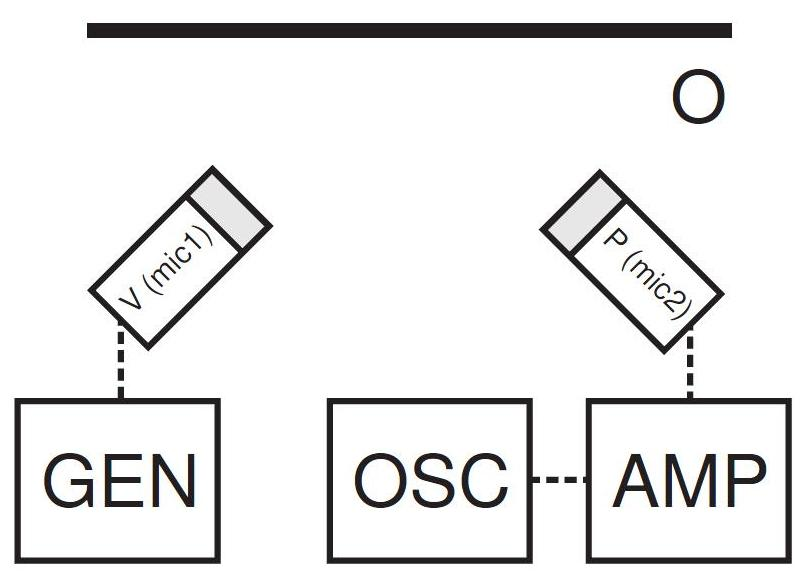
\includegraphics[width=.53\linewidth]{att/s_zakon.jpg}
	  \caption{Schéma zapojení pro ověřování platnosti zákonu odrazu (GEN generátor, OSC oscilátor, AMP zesilovač, P a V mikrofony, O odrazová deska) \cite{bib:zadani}.}
	  \label{fig:s_zakon_odrazu}
	\end{minipage}%
	\hfill
	\begin{minipage}{.45\textwidth}
	  \centering
	  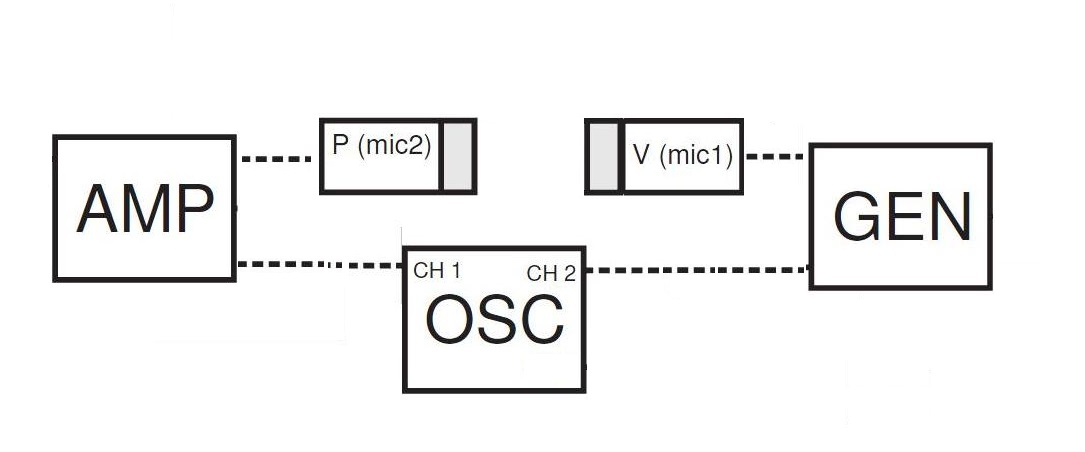
\includegraphics[width=.9\linewidth]{att/s_rychlost.jpg}
	  \caption{Schéma zapojení pro měření rychlosti zvuku (GEN generátor, OSC oscilátor, AMP zesilovač, P a V mikrofony) \cite{bib:repo}.}
	  \label{fig:s_rychlost_zvuku}
	\end{minipage}
	\end{figure}

	\subsubsection{Dopplerův jev}
		Pro tuto úlohu jsme využívali zapojení dle schématu \ref{fig:s_doppler}. Pohyb přijímače/vysílače po dráze zajišťoval malý vozík na baterky nastavený tak, aby pokud možno udržoval na konkrétních úsecích konstantní rychlost. Pro každou za čtyř skupin měření jsme zaznamenali klidovou frekvenci $f_0$ při odpovídající vzdálenosti přijímače a vysílače, změřili vzdálenost $s$, na které jsme stopovali pohyb vozíku, a uvažovali rychlost zvuku změřenou v druhé úloze. Následně jsme pro každou ze čtyř konfigurací (pohyb vysílače/přijímače od a k druhému) měřili čas $t$, za jaký vozík urazil vzdálenost $s$, a během tohoto pohybu odečetli z čítače Tesla hodnotu frekvence z přijímače. 

	\subsubsection{Difrakce a interference zvuku}
		Zapojení aparatury proběhlo podle schématu na obrázku \ref{fig:s_difrakce}, mřížka byla umístěna na papírovém úhloměru kolmo k desce lavice. Před vlastním měřením pomocí ultrazvuku jsme zaznamenali rozmístění štěrbin na mřížce a vzdálenost přijímače od středu úhloměru, ve které probíhala měření. Při vlastním měření jsme zaznamenávali intenzitu signálu $A$ v dané vzdálenosti od mřížky o $N$ odkrytých štěrbinách (pro $N = 1,2,5$) v závislosti na úhlu $\alpha$ k ose vysílače s parabolou. Pro $N=1, 2$ jsme se pouze snažili nalézt minima a maxima signálu, pro $N=5$ jsme pak učinili více měření i pro mezihodnoty.
		
	\begin{figure}
	\begin{minipage}{.45\textwidth}
		\centering
		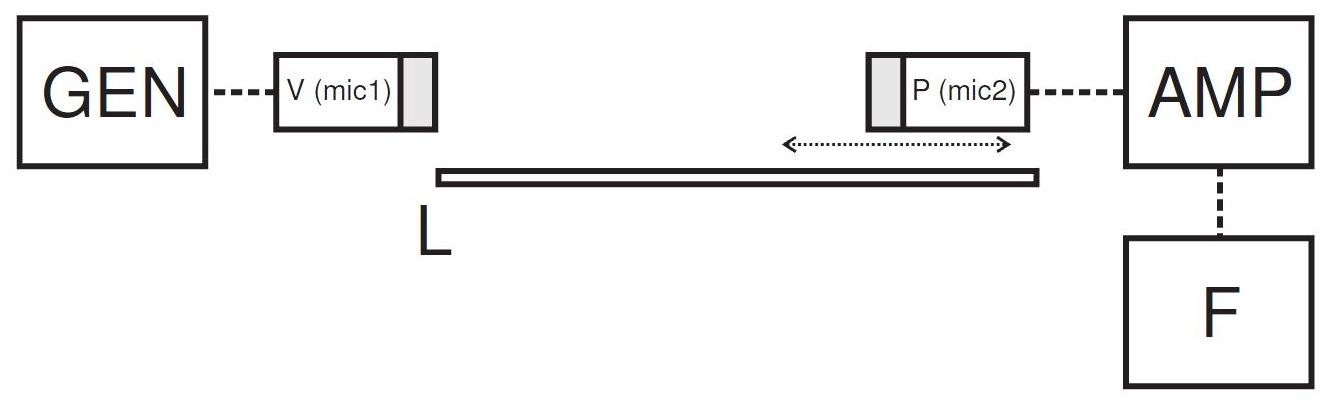
\includegraphics[width=1\linewidth]{att/s_doppler.jpg}
		\caption{Schéma zapojení pro měření Dopplerova jevu (GEN generátor, AMP zesilovač, P a V mikrofony, F čítač Tesla, L pojezdová lavice) \cite{bib:zadani}.}
		\label{fig:s_doppler}
	\end{minipage}
	\centering
	\hfill
	\begin{minipage}{.45\textwidth}
		\centering
		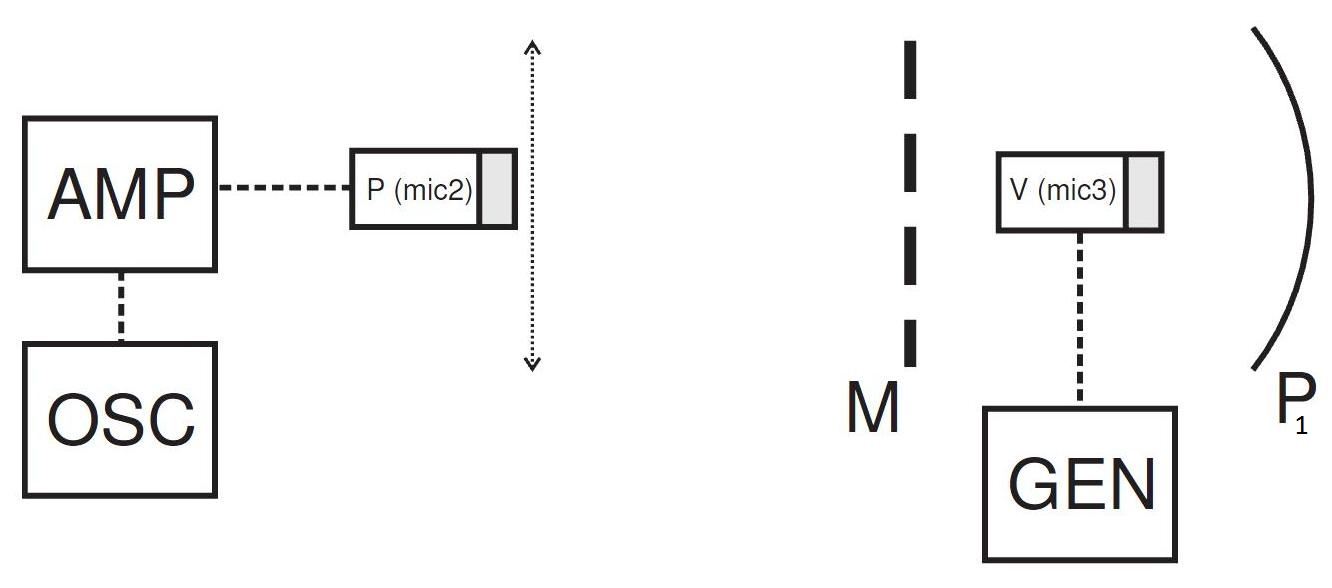
\includegraphics[width=.73\linewidth]{att/s_difrakce.jpg}
		\caption{Schéma zapojení pro měření difrakce (GEN generátor, OSC oscilátor, AMP zesilovač, P a V mikrofony, $P_1$ parabola vysílače, M mřížka) \cite{bib:zadani}.}
		\label{fig:s_difrakce}
	\end{minipage}%
	
	\end{figure}

\subsection{Naměřené hodnoty}

	\subsubsection{Zákon odrazu}
		Naměřené hodnoty jsou uvedeny v tabulce \ref{tab:zakon_odrazu} a vyneseny spolu s ilustračními parabolickými fity v grafu \ref{fig:g_zakon_odrazu}.
	
	\begin{table}[h]
	\begin{center}
	\begin{tabular}{|r|r|r|r||r|r|r|r||r|r|r|r|}
	\hline
	       $\alpha$ [$^\circ$] & $\beta$ [$^\circ$] & $A$ [V] & $\gamma$ [$^\circ$] & $\alpha$ [$^\circ$] & $\beta$ [$^\circ$] & $A$ [V] & $\gamma$ [$^\circ$] & $\alpha$ [$^\circ$] & $\beta$ [$^\circ$] & $A$ [V] & $\gamma$ [$^\circ$]\\\hline \hline
	       $-45$ & $5$ & $34,5$ & $-40$ & $-30$ & $0$ & $46,0$ & $-30$ & $-60$ & $80$ & $47,6$ & $20$\\\hline
	       $-45$ & $15$ & $42,1$ & $-30$ & $-30$ & $10$ & $48,7$ & $-20$ & $-60$ & $70$ & $48,3$ & $10$\\\hline
	       $-45$ & $25$ & $44,6$ & $-20$ & $-30$ & $20$ & $50,8$ & $-10$ & $-60$ & $60$ & $48,8$ & $0$\\\hline
	       $-45$ & $35$ & $48,2$ & $-10$ & $-30$ & $30$ & $51,3$ & $0$ & $-60$ & $50$ & $48,0$ & $-10$\\\hline
	       $-45$ & $45$ & $50,7$ & $0$ & $-30$ & $40$ & $50,2$ & $10$ & $-60$ & $40$ & $47,5$ & $-20$\\\hline
	       $-45$ & $55$ & $49,3$ & $10$ & $-30$ & $50$ & $47,4$ & $20$ & $-60$ & $30$ & $42,8$ & $-30$\\\hline
	       $-45$ & $65$ & $44,8$ & $20$ & $-30$ & $60$ & $44,1$ & $30$ & $-60$ & $20$ & $37,0$ & $-40$\\\hline
	
	\end{tabular}
	\caption{Zákon odrazu. Ve všech třech sadách měření je $\alpha$ úhel vysílače, $\beta$ úhel přijímače. Oba úhly jsou brány vůči kolmici k odrazové desce. Úhel $\gamma$ je rozdíl jejich absolutních hodnot a $A$ velikost přijímaného signálu.}
	\label{tab:zakon_odrazu}
	\end{center}
	\end{table}
	
	\subsubsection{Měření rychlosti zvuku}
		Naměřené hodnoty jsou uvedeny v tabulce \ref{tab:rychlost_zvuku} a proloženy lineárním fitem v grafu \ref{fig:g_rychlost_zvuku}.
		
	\begin{table}[h]
	\begin{center}
	\begin{tabular}{|r|r|}
	\hline
         $s$ [cm] & $t$ [$\mu$s] \\\hline \hline
         $10$ & $350$ \\\hline
         $15$ & $465$ \\\hline
         $20$ & $628$ \\\hline
         $25$ & $795$ \\\hline
         $30$ & $967$ \\\hline
         $35$ & $1080$ \\\hline
         $40$ & $1230$ \\\hline
         $45$ & $1390$ \\\hline
         $50$ & $1530$ \\\hline
         $55$ & $1690$ \\\hline
         $60$ & $1830$ \\\hline
         $65$ & $1990$ \\\hline
         $70$ & $2140$ \\\hline
	
	\end{tabular}
	\caption{Měření rychlosti zvuku. Časy $t$, za které zvuk urazil vzdálenosti $s$.}
	\label{tab:rychlost_zvuku}
	\end{center}
	\end{table}
	
	\subsubsection{Měření vzdálenosti}
		Naměřené hodnoty jsou uvedeny v tabulce \ref{tab:mereni_vzdalenosti}.
		
	\begin{table}[h]
	\begin{center}
	\begin{tabular}{|r|r|r|r|r|r|r|r|}
	\hline
     $s_r$ [cm] & $t_1$ [$\mu$s] & $t_2$ [$\mu$s] & $t_3$ [$\mu$s] & $t_c$ [$\mu$s] & $\sigma_t$ [$\mu$s] & $s_v$ [cm] & $\sigma_s$ [cm] \\\hline \hline
     $10$ & $741$ & $690$ & $685$ & $705$ & $18$ & $24,3$ & $0,7$ \\\hline
     $20$ & $1260$ & $1240$ & $1220$ & $1240$ & $12$ & $42,8$ & $0,7$ \\\hline
     $30$ & $1860$ & $1790$ & $1800$ & $1817$ & $22$ & $62,7$ & $1,2$ \\\hline
     $40$ & $2410$ & $2370$ & $2390$ & $2390$ & $12$ & $82,5$ & $1,3$ \\\hline
     $50$ & $2940$ & $2990$ & $2970$ & $2967$ & $15$ & $102,4$ & $1,6$ \\\hline
	
	\end{tabular}
	\caption{Měření vzdálenosti. Vzdálenost $s_r$ je změřená svinovacím metrem, $t_1$, $t_2$, $t_3$ časy, za které zvuk tuto vzdálost urazil. Aritmetický průměr těchto časů je $t_c$, $\sigma_t$ chyba tohoto průměru. Vzdálenost spočítaná pomocí rychlosti zvuku z předchozí úlohy je $s_v$, $\sigma_s$ její chyba \cite{bib:chyby}.}
	\label{tab:mereni_vzdalenosti}
	\end{center}
	\end{table}

	\subsubsection{Dopplerův jev}
		Naměřené hodnoty jsou uvedeny v tabulkách \ref{tab:doppler_k_sobe} a \ref{tab:doppler_od_sebe}.
		
	\begin{table}[h]
	\catcode`\-=12 % HAX na enable cline v českym bable
	\begin{center}
	\begin{tabular}{|r|r|r||r|r|c|r|r|r||r|r|}
    \cline{1-5} \cline{7-11}
 	
 	$t$ [s] & $v$ [m/s] & $f_m$ [kHz] & $v$ [m/s] & $\sigma_v$ [m/s]  && $t$ [s] & $v$ [m/s] & $f_m$ [kHz] & $v$ [m/s] & $\sigma_v$ [m/s]   \\\cline{1-5} \cline{7-11}
	$1,22$ & $0,41$ & $45,6$ & $0,44$ & $0,01$ 						  && $1,03$ & $0,49$ & $44,9$ & $0,42$ & $0,02$ 						\\\cline{1-5} \cline{7-11}
	$1,19$ & $0,42$ & $45,1$ & $f_m$ [kHz] & $\sigma_{f_m}$ [kHz] 	  && $1,19$ & $0,42$ & $45,4$ & $f_m$ [kHz] & $\sigma_{f_m}$ [kHz]		\\\cline{1-5} \cline{7-11}
	$1,18$ & $0,42$ & $46,3$ & $45,8$ & $0,3$					 	  && $1,23$ & $0,41$ & $46,2$ & $45,3$ & $0,4$ 							\\\cline{1-5} \cline{7-11}
	$1,08$ & $0,46$ & $45,2$ & $f_v$ [kHz] & $\sigma_{f_v}$ [kHz]     && $1,24$ & $0,40$ & $44,1$ & $f_v$ [kHz] & $\sigma_{f_v}$ [kHz] 		\\\cline{1-5} \cline{7-11}
	$1,09$ & $0,46$ & $46,9$ & $45,2$ & $0,7$                         && $1,26$ & $0,40$ & $46,1$ & $40,5$ & $0,6$ 							\\\cline{1-5} \cline{7-11}
 	 
	\end{tabular}
	\caption{Měření Dopplerova jevu při pohybu přijímače (levá část) a vysílače (pravá část) směrem k sobě. Čas $t$ je doba jak dlouho jel vozík po vyměřené dráze $s = (0,5 \pm 0,001)$ m, $v$ jeho spočítaná rychlost, $f_m$ frekvence měřená čítačem, $f_v$ teoreticky spočítaná frekvence. Pro výpočty uvažujeme $v_z = (345 \pm 5)$ m/s, $f_{0l} = (45,1 \pm 0,7)$ kHz a $f_{0r} = (40,5 \pm 0,6)$ kHz \cite{bib:chyby}.
	}
	\label{tab:doppler_k_sobe}
	\end{center}
	\end{table}
	
	
	\begin{table}[h]
	\catcode`\-=12 % HAX na enable cline v českym bable
	\begin{center}
	\begin{tabular}{|r|r|r||r|r|c|r|r|r||r|r|}
	\cline{1-5} \cline{7-11}
 	
 	$t$ [s] & $v$ [m/s] & $f_m$ [kHz] & $v$ [m/s] & $\sigma_v$ [m/s] && $t$ [s] & $v$ [m/s] & $f_m$ [kHz] & $v$ [m/s] & $\sigma_v$ [m/s] 	\\\cline{1-5} \cline{7-11}
	$1,14$ & $0,44$ & $39,73$ & $0,43$      & $0,02$                 && $1,08$ & $0,46$ & $41,7$ & $0,39$ & $0,04$ 							\\\cline{1-5} \cline{7-11}
	$1,09$ & $0,46$ & $39,72$ & $f_m$ [kHz] & $\sigma_{f_m}$ [kHz]   && $1,18$ & $0,42$ & $40,5$ & $f_m$ [kHz] & $\sigma_{f_m}$ [kHz]  		\\\cline{1-5} \cline{7-11}
	$1,39$ & $0,36$ & $39,71$ & $39,7$     & $0,1$                 && $1,16$ & $0,43$ & $40,8$ & $40,7$ & $0,3$ 							\\\cline{1-5} \cline{7-11}
	$1,11$ & $0,45$ & $39,73$ & $f_v$ [kHz] & $\sigma_{f_v}$ [kHz]   && $2,01$ & $0,25$ & $40,5$ & $f_v$ [kHz] & $\sigma_{f_v}$ [kHz]  		\\\cline{1-5} \cline{7-11}
	$1,19$ & $0,42$ & $39,71$ & $39,7$      & $0,6$                  && $1,33$ & $0,38$ & $40,2$ & $40,4$ & $0,6$ 							\\\cline{1-5} \cline{7-11}
	     
	\end{tabular}
	\caption{Měření Dopplerova jevu při pohybu přijímače (levá část) a vysílače (pravá část) směrem od sebe. Čas $t$ je doba jak dlouho jel vozík po vyměřené dráze $s = (0,5 \pm 0,001)$ m, $v$ jeho spočítaná rychlost, $f_m$ frekvence měřená čítačem, $f_v$ teoreticky spočítaná frekvence. Pro výpočty uvažujeme $v_z = (345 \pm 5)$ m/s, $f_{0l} = (39,8 \pm 0,6)$ kHz a $f_{0r} = (40,5 \pm 0,6)$ kHz \cite{bib:chyby}.
	}
	\label{tab:doppler_od_sebe}
	\end{center}
	\end{table}
	
	\subsubsection{Difrakce a interference zvuku}
		Naměřené hodnoty jsou uvedeny v tabulkách \ref{tab:difrakce_n1}, \ref{tab:difrakce_n2} a \ref{tab:difrakce_n5} a vyneseny do grafů \ref{fig:g_difrakce_n1}, \ref{fig:g_difrakce_n2} a \ref{fig:g_difrakce_n5}.
	
	\begin{table}
	\parbox{.33\linewidth}{
	\centering
	\begin{tabular}{|r|r|}
	\hline
	$\alpha$ [$^\circ$]   &   $A$ [V] \\\hline \hline
	$18$   &   $5,89$ \\\hline
	$10$   &   $2,12$ \\\hline
	$-2$   &   $7,39$ \\\hline
	$-7$   &   $2,24$ \\\hline
	$-16$   &   $5,16$ \\\hline
	
	\end{tabular}
	
	\caption{Měření difrakce. Závislost intenzity signálu $A$ na úhlu vůči ose vysílače $\alpha$ pro počet štěrbin $N=1$.}
	\label{tab:difrakce_n1}
	}
	%\hfill
	\parbox{.33\linewidth}{
	\centering
	\begin{tabular}{|r|r|}
	\hline
	$\alpha$ [$^\circ$]   &   $A$ [V] \\\hline \hline
	$15$   &   $2,25$ \\\hline
	$10$   &   $3,37$ \\\hline
	$5$   &   $3,48$ \\\hline
	$0$   &   $4,02$ \\\hline
	$-5$   &   $3,60$ \\\hline
	$-10$   &   $3,79$ \\\hline
	$-15$   &   $2,22$ \\\hline
	$-20$   &   $2,10$ \\\hline
	
	\end{tabular}
		
	\caption{Měření difrakce. Závislost intenzity signálu $A$ na úhlu vůči ose vysílače $\alpha$ pro počet štěrbin $N=2$.}
	\label{tab:difrakce_n2}
	}
	\hfill
	\parbox{.33\linewidth}{
	\centering
	\begin{tabular}{|r|r|}
	\hline
	$\alpha$ [$^\circ$]   &   $A$ [V] \\\hline \hline
	$18,5$   &   $2,23$ \\\hline
	$17$   &   $3,59$ \\\hline
	$15$   &   $8,09$ \\\hline
	$11,5$   &   $4,09$ \\\hline
	$8,5$   &   $1,89$ \\\hline
	$7,5$   &   $6,72$ \\\hline
	$5$   &   $7,36$ \\\hline
	$2,5$   &   $7,56$ \\\hline
	$0$   &   $2,07$ \\\hline
	$-2,5$   &   $9,08$ \\\hline
	$-5$   &   $1,25$ \\\hline
	$-7,5$   &   $6,59$ \\\hline
	$-9$   &   $1,59$ \\\hline
	$-13$   &   $8,47$ \\\hline
	
	\end{tabular}
	\caption{Měření difrakce. Závislost intenzity signálu $A$ na úhlu vůči ose vysílače $\alpha$ pro počet štěrbin $N=5$.}
	\label{tab:difrakce_n5}	
	}
	
	\end{table}

\subsection{Diskuse}	
    
    \subsubsection{Zákon odrazu}
    	Zákon odrazu se podařilo úspěšně dokázat a výsledky odpovídají teoretickým předpokladům pro všechny tři úhly odrazu (maxima dosahuje velikost signálu při $\gamma = 0\ ^\circ$). Měření by však mohlo být mnohem přesnější. K největším nepřesnostem však vedl fakt, že intenzita signálu velmi záležela na orientaci vysílače a přijímače. Úhel stojanů s mikrofony ke kolmici desky se dal určit relativně dobře, ale téměř nešlo zjistit, kam přesně oba mikrofony ukazují. Tento fakt jsme se snažili vykompenzovat pečlivým otáčením přijímače v každém úhlu a hledáním maximální velikosti signálu - té však v některých místech dosahoval v poloze, kdy zcela jistě nemířil na bod odrazu na desce. Nepřesnosti se tak mohly pohybovat až v desítkách stupňů. Měření by šlo zpřesnit použitím kvalitnějších směrových mikrofonů nebo světelným značením směru, kterým jsou mikrofony nasměrovány. 

	\subsubsection{Měření rychlosti zvuku}
		Rychlost zvuku jsme určili z lineárního proložení naměřených dat na $v_z = (345 \pm 5)$ m/s při teplotě v místnosti $t=23\ ^\circ C$, čemuž odpovídá hodnota $334,97$ m/s, kterou jsme spočítali dle vzorce \ref{eq:teorie_rychlost_zvuku} v teoretickém úvodu. Teoreticky určená rychlost při dané teplotě tedy leží v intervalu chyb námi změřené hodnoty a naše měření můžeme označit za úspěšné. K nepřesnostem vedl fakt, že na osciloskopu nešlo vzhledem k jeho postupnému nástupu jednoznačně určit, kdy signál začal. Snažili jsme se alespoň umisťovat druhý kurzor konzistentně do jedné polohy vzhledem ke křivce signálu a tuto systematickou odchylku následně eliminovat konstantním členem lineárního proložení. 
	
	\subsubsection{Měření vzdáleností}
		Měření vzdálenosti metodou sonaru se nám na první pohled příliš nezdařilo, jelikož svinovacím metrem naměřené hodnoty neleží po zdvojnásobení v intervalu statistických chyb hodnot naměřených ultrazvukem. K nepřesnostem vedlo, že stojany přijímače a vysílače svíraly nenulový úhel $\alpha$ vzhledem k ose odrazové plochy a dráha zvuku tak nebyla pouhým dvojnásobkem naměřené vzdálenosti, ale o trochu větší. Měřená vzdálenost od odrazové desky byla také spíše podhodnocována vzhledem ke špatně měřitelné poloze mikrofonů ve stojanech. Zahrneme-li tyto systematické chyby v řádu jednotek centimetrů, leží už metrem naměřené hodnoty v chybových intervalech výsledků. Nic to však nemění na tom, že je metoda sonaru v našem provedení méně přesná než změření vzdálenosti svinovacím metrem. Výsledky by se daly zpřesnit umístěním vysílače a přijímače blíže k sobě, přesnějším změřením vzdálenosti obou od odrazové desky a provedením většího počtu měření pro každou vzdálenost.

	\subsubsection{Dopplerův jev}
		Měření Dopplerova jevu bylo nepřesné z několika důvodů. Změření změny frekvence je závislé na přesném určení okamžité rychlosti vozíku a tím pádem i na tom, jak dobře se vozík pohybuje konstantní rychlostí na měřeném úseku. Dále jsme zjistili, že ve vzdálenostech vysílač/přijímač větších než 70 centimetrů kolísá frekvence na čítači v řádu jednotek, což umisťuje chyby o dva řády výše, než kde chceme pozorovat změnu vlivem sledovaného jevu. Ve snaze zmenšit chyby způsobené těmito příčinami jsme volili vzdálenost, na které jsme stopovali pohyb vozíku, na 50 cm. Pokud bychom volili menší vzdálenost, dosahovala by chyba měření časů příliš velkých hodnot vzhledem k velikosti měřené doby. Ta by se dala prodloužit zpomalením vozíku, ale to by opět negativně ovlivňovalo velikost námi měřeného Dopplerova jevu, který je pro menší rychlosti hůře měřitelný. 
		
		Pro měření frekvencí $f_{0r}$ a $f_{0l}$ čítačem Tesla jsme statistickou chybu určili pomocí aritmetického průměru deseti měření této klidové frekvence. Statistická chyba vypočtené frekvence $f_v$ vychází podstatně menší, ale vzhledem k systematickým chybám diskutovaným v předchozím odstavci můžeme její reálnou chybu rozhodně zespoda odhadnout chybou klidové frekvence $f_{0r/l}$ pro danou konfiguraci měření. Ve stejných řádech se pak pohybuje i statistická chyba frekvence $f_m$ měřené čítačem Tesla.
		
		Podle teoretických výpočtů by se při pohybu vysílače a přijímače k sobě měla měřená frekvence zvyšovat a tím pádem by mělo platit $f_m = f_v > f_{0l/r}$. Stejně tak by se při pohybu obou mikrofonů od sebe měla frekvence zmenšovat a tím pádem by mělo platit $f_m = f_v < f_{0l/r}$. Předpokládané chování námi naměřené hodnoty nepotvrzují ani nevyvrací, jelikož je průnik chybových intervalů frekvencí $f_{m/v}$ a $f_{0l/r}$ vždy neprázdný i při spodním odhadu systematické chyby měření.
		
		Kromě v prvním odstavci diskutovaných vlivů je třeba zmínit, že k chybám mohly přispět problémy probírané při diskusi měření úhlu odrazu, v praktiku zároveň probíhající experimenty se zvukem vysokých frekvencí, zatěžování vozíku kabely mikrofonů, jeho nedostatečná rychlost nebo špatně sesynchronizované odečítání frekvence na čítači Tesla s pohybem vozíku po dráze. Celý experiment by se dal zpřesnit, například měřením okamžité rychlosti vozíku jinou metodou, ideálně synchronizovanou s odečítáním frekvence měřené na čítači. Nutností pro smysluplné měření Dopplerova jevu se jeví přizpůsobení amplitudy a frekvence zdroje tak, aby se chyba určení klidové $f_0$ zmenšila z desítek či stovek Hz alespoň na jednotky. 

	\subsubsection{Difrakce a interference zvuku}
		Oproti návodu \cite{bib:zadani} jsme tuto úlohu prováděli s menší vzdáleností přijímače od mřížky $d = 50$ cm, jelikož ve větších vzdálenostech byla měřená intenzita příliš nízká a kolísala. Nevýhodou tohoto postupu je, že se v bližší vzdálenosti mnohem více projevuje chyba umístění. I tak ale poskytovala tato konfigurace lepší výsledky. I přes relativně velkou statistickou chybu se nám podařilo najít minima a maxima, grafy bodů rámcově odpovídají difrakčním obrazcům.
		
\section{Závěr}
	Úspěšně jsme ověřili, že platí zákon odrazu pro ultrazvukové vlny a změřili jsme rychlost zvuku ve vzduchu s dostačující přesností. Vyzkoušeli a zhodnotili jsme metodu měření vzdálenosti principem sonaru a proměřili difrakci na mřížce pro různý počet štěrbin. Dopplerův jev se nám nepodařilo prokázat, ale naše výsledky ho nevyvrací.


\section {Použitá literatura}
% --- Literatura a reference -------------------------------------------
\begingroup
\renewcommand{\section}[2]{}

\begin{thebibliography}{9}
\bibitem{bib:zadani} Kolektiv KF, \emph{Návod k úloze: Studium ultrazvukových vln} [Online], [cit. \today] \newline 
http://praktikum.fjfi.cvut.cz/pluginfile.php/123/mod\_resource/content/2/8\_Sonar.pdf

\bibitem{bib:repo} Kolektiv autorů, \emph{Repozitář zdrojů k praktiku} [Online] [cit. \today] \newline https://github.com/roesel/praktika

%\bibitem{bib:navody} Kolektiv KF, \emph{Návody k přístrojům} [Online], [cit. \today] \newline http://praktikum.fjfi.cvut.cz/documents/chybynav/navody-o.pdf

\bibitem{bib:chyby} Kolektiv KF, \emph{Chyby měření} [Online], [cit. \today] \newline http://praktikum.fjfi.cvut.cz/documents/chybynav/chyby-o.pdf

\end{thebibliography}
\endgroup
% ----------------------------------------------------------------------

\section{Přílohy}

\subsection{Domácí příprava}
	Domácí příprava je přiložena k protokolu.

\subsection{Statistické zpracování dat}
	Pro statistické zpracování využíváme aritmetického průměru:
	\begin{equation} \label{eq:aritmeticky_prumer}
	\overline{x} = \frac{1}{n}\sum\limits_{i=1}^{n}x_i
	\end{equation}
	
	jehož chybu spočítáme jako 
	\begin{equation} \label{eq:chyba_aritmetickeho_prumeru}
	\sigma_0 = \sqrt{\frac{1}{n(n-1)} \sum\limits_{i=1}^{n}\left( x_i - \overline{x} \right)^2 },
	\end{equation}
	
	kde $ x_i $ jsou jednotlivé naměřené hodnoty, $ n $ je počet měření, $ \overline{x} $ aritmetický průměr a $ \sigma_0 $ jeho chyba \cite{bib:chyby}.
	
	Při nepřímém měření počítáme hodnotu s chybou dle následujících vztahů:
	\begin{equation}
	u = f(x, y, z, \ldots)
	\end{equation}
	\begin{displaymath}
	x = (\overline{x} \pm \sigma_x), \qquad
	y = (\overline{y} \pm \sigma_y), \qquad
	z = (\overline{z} \pm \sigma_z), \qquad
	\ldots,
	\end{displaymath}
	
	kde $ u $ je veličina, kterou určujeme nepřímo z měřených veličin $ x, y, z, \ldots $ 
	
	Pak
	\begin{displaymath}
	\overline{u} = f(\overline{x}, \overline{y}, \overline{z}, \ldots)
	\end{displaymath}
	\begin{equation}\label{eq:chyba_neprime_mereni}
	\sigma_u = \sqrt{\left( \frac{\partial f}{\partial x} \right)^2 \sigma^2_x + \left( \frac{\partial f}{\partial y} \right)^2 \sigma^2_y + \left( \frac{\partial f}{\partial z} \right)^2 \sigma^2_z + \ldots}
	\end{equation}
	\begin{displaymath}
	u = (\overline{u} \pm \sigma_ u),
	\end{displaymath}
\newpage
\subsection{Grafy}
	
	\begin{figure}[h]
	\begin{center}
	    %\vspace*{-1cm}
		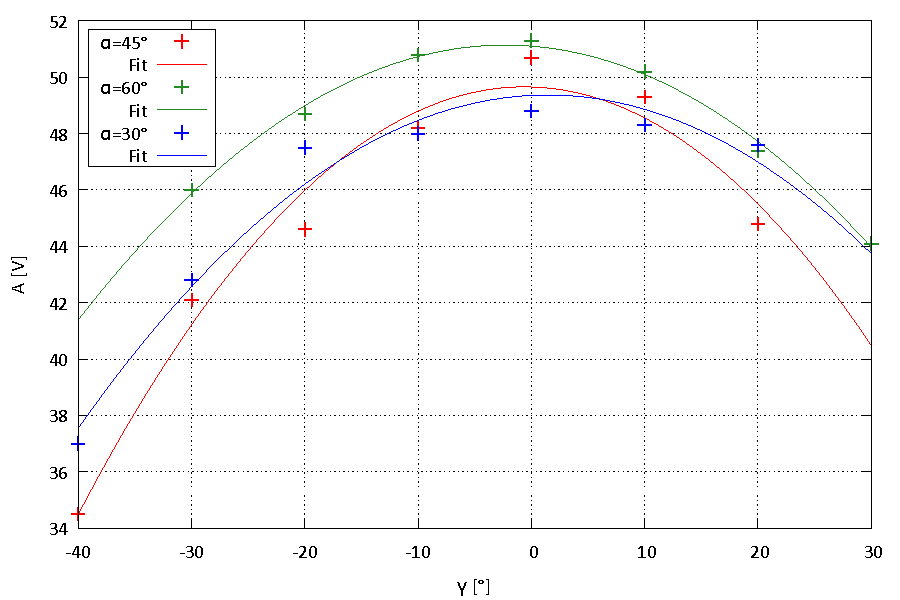
\includegraphics[width=\linewidth]{../gnuplot/8_sonar_zk_out.pdf}
	    %\vspace*{-1cm}
		\caption{Graf hodnot ověřování platnosti zákonu odrazu pro ultrazvukové vlny.}
		\label{fig:g_zakon_odrazu}
	\end{center}
	\end{figure}
	
	\begin{figure}[p]
	\begin{center}
		\vspace*{-1cm}
		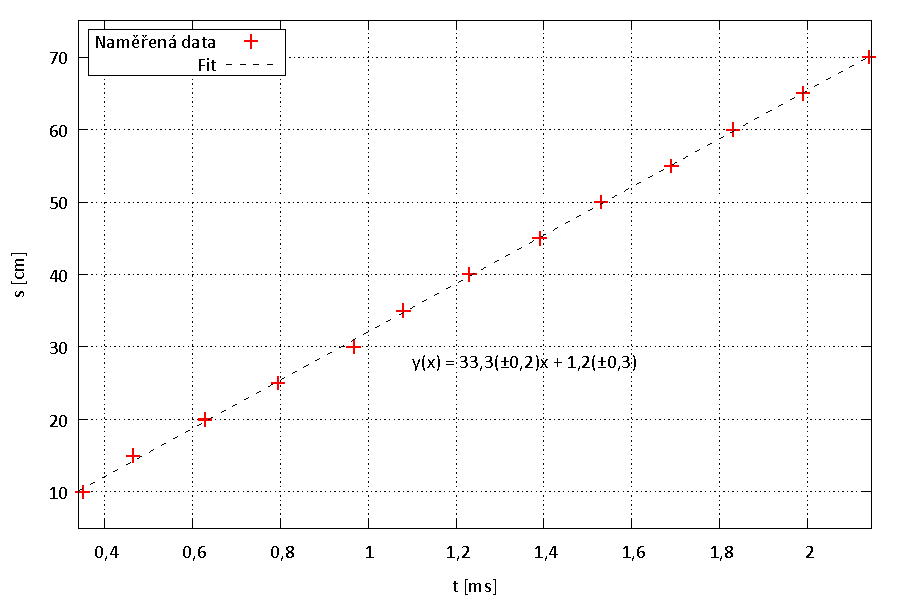
\includegraphics[width=\linewidth]{../gnuplot/8_sonar_vz_out.pdf}
		\vspace*{-1cm}    
		\caption{Graf měření rychlosti zvuku ve vzduchu. Proloženo lineárním fitem.}
		\label{fig:g_rychlost_zvuku}
	\end{center}
	\end{figure}
	
	\begin{figure}[p]
	\begin{center}
	    \vspace*{-1cm}
	    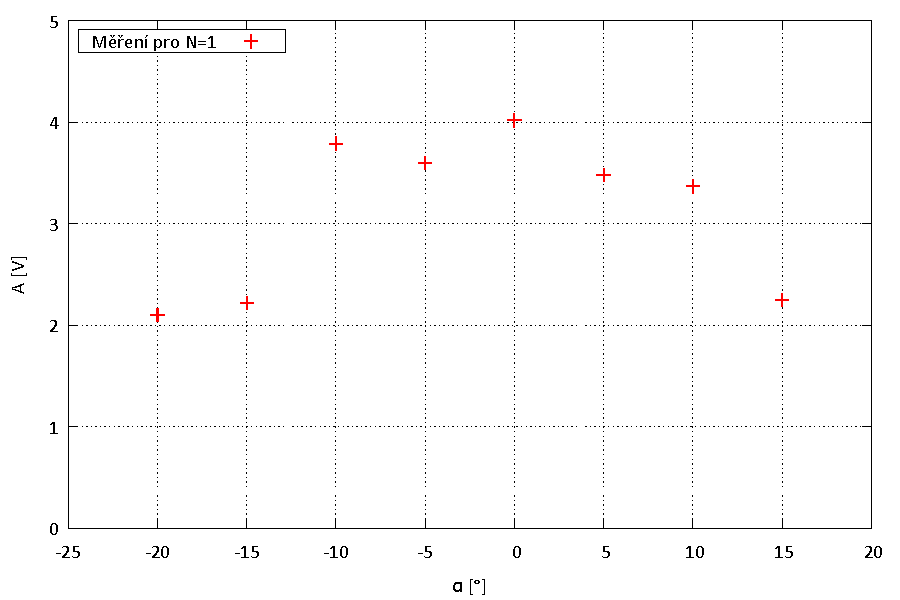
\includegraphics[width=\linewidth]{../gnuplot/8_sonar_if_1_out.pdf}
	    \vspace*{-1cm}    
		\caption{Graf měření difrakce ultrazvukových vln pro počet štěrbin $N=1$.}
		\label{fig:g_difrakce_n1}
	\end{center}
	\end{figure}

	\begin{figure}[p]
	\begin{center}
	    \vspace*{-1cm}
	    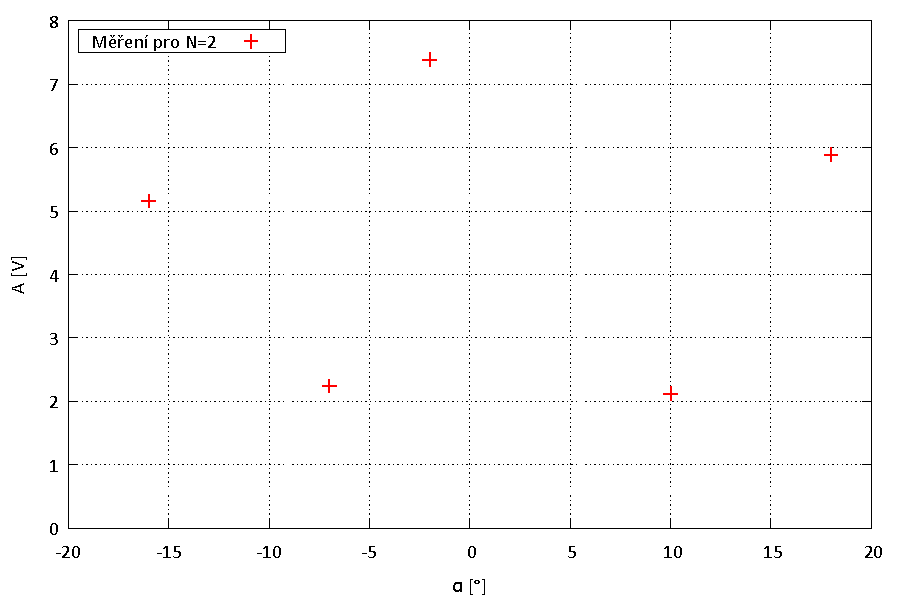
\includegraphics[width=\linewidth]{../gnuplot/8_sonar_if_2_out.pdf}
	    \vspace*{-1cm}    
		\caption{Graf měření difrakce ultrazvukových vln pro počet štěrbin $N=2$.}
		\label{fig:g_difrakce_n2}
	\end{center}
	\end{figure}
	
	\begin{figure}[p]
	\begin{center}
	    \vspace*{-1cm}
	    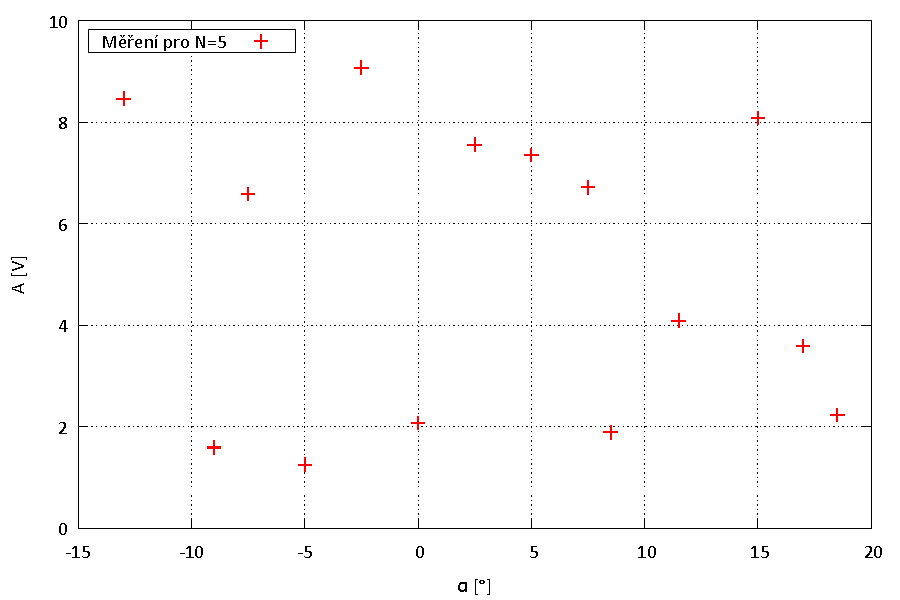
\includegraphics[width=\linewidth]{../gnuplot/8_sonar_if_3_out.pdf}
	    \vspace*{-1cm}    
		\caption{Graf měření difrakce ultrazvukových vln pro počet štěrbin $N=5$.}
		\label{fig:g_difrakce_n5}
	\end{center}
	\end{figure}	
	
% --- The funs ---------------------------------------------------------
\newpage
\subsection{Nepodařené fity}
	
	\begin{figure}[h]
	\begin{center}
	    %\vspace*{-1cm}
		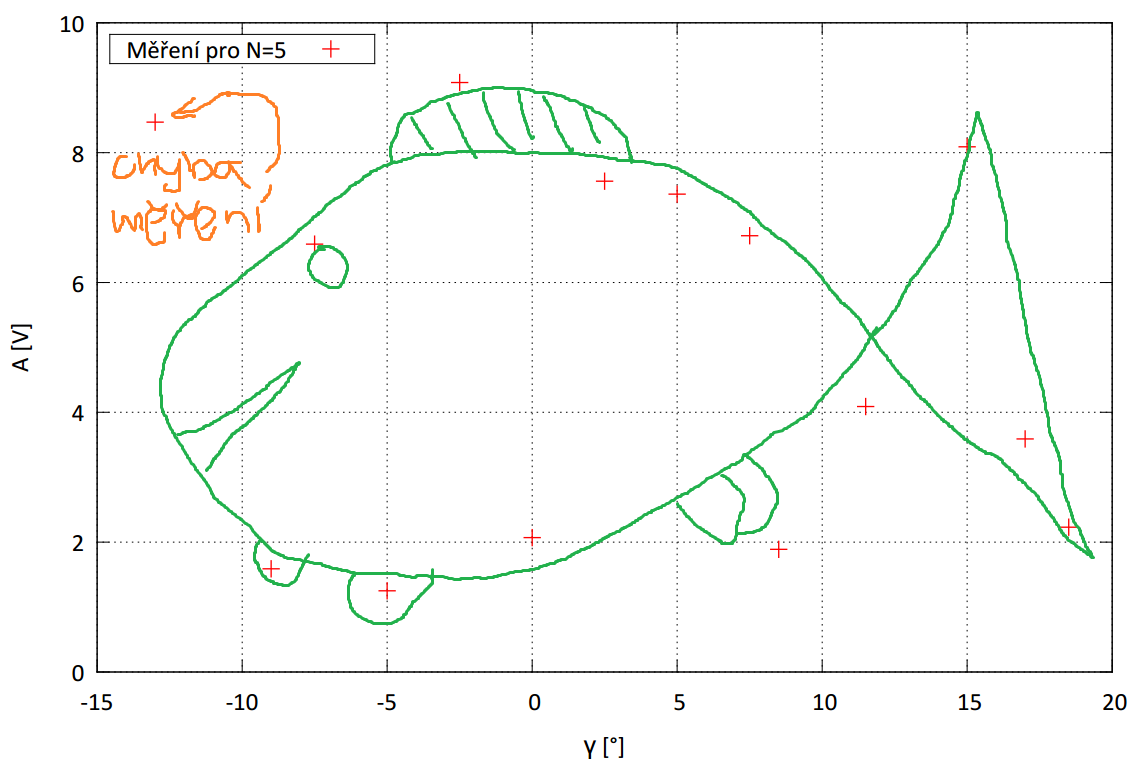
\includegraphics[width=\linewidth]{att/ryba.png}
	    %\vspace*{-1cm}
		\caption{Body jsme proložili speciální \emph{rybou měření} a je při tom evidentní chyba měření, která byla příliš velká.}
		\label{fig:g_fun_1}
	\end{center}
	\end{figure}
	
	\begin{figure}[p]
	\begin{center}
		\vspace*{-1cm}
		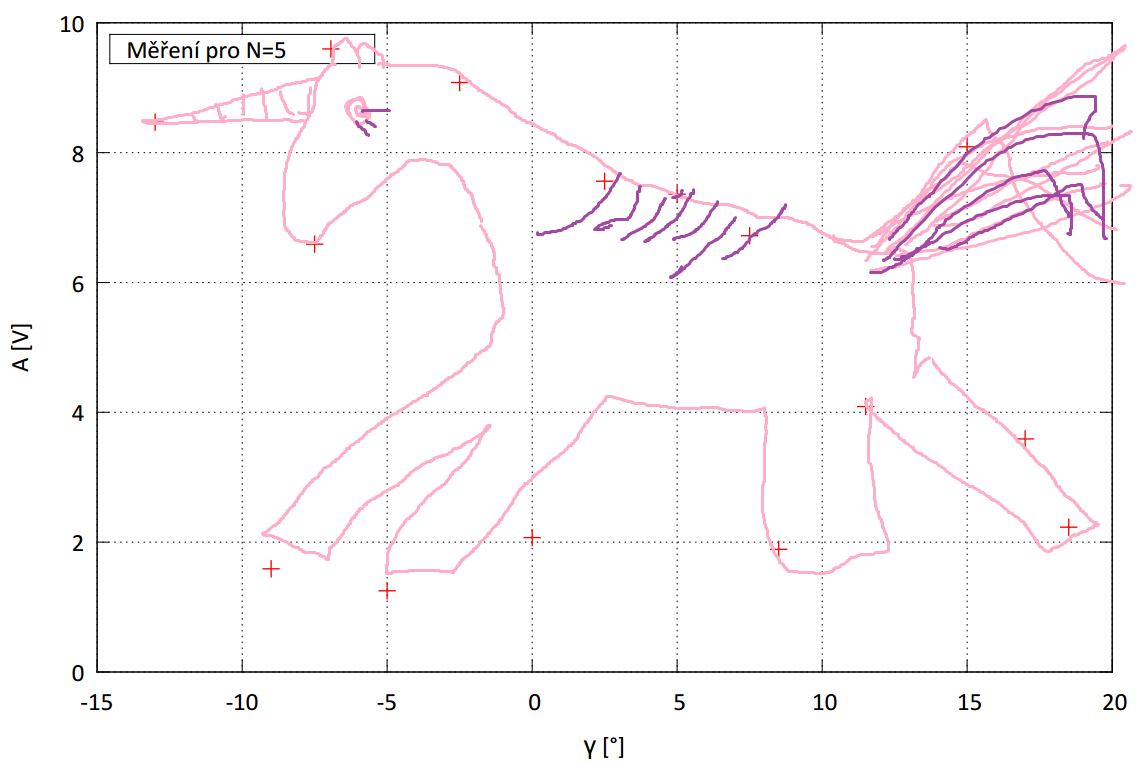
\includegraphics[width=\linewidth]{att/jednorozec.png}
		\vspace*{-1cm}
		\caption{Funkce \emph{Friendship is magic} také zcela nevyhovovala požadavkům.}
		\label{fig:g_fun_2}
	\end{center}
	\end{figure}
	
	\begin{figure}[p]
	\begin{center}
	    \vspace*{-1cm}
	    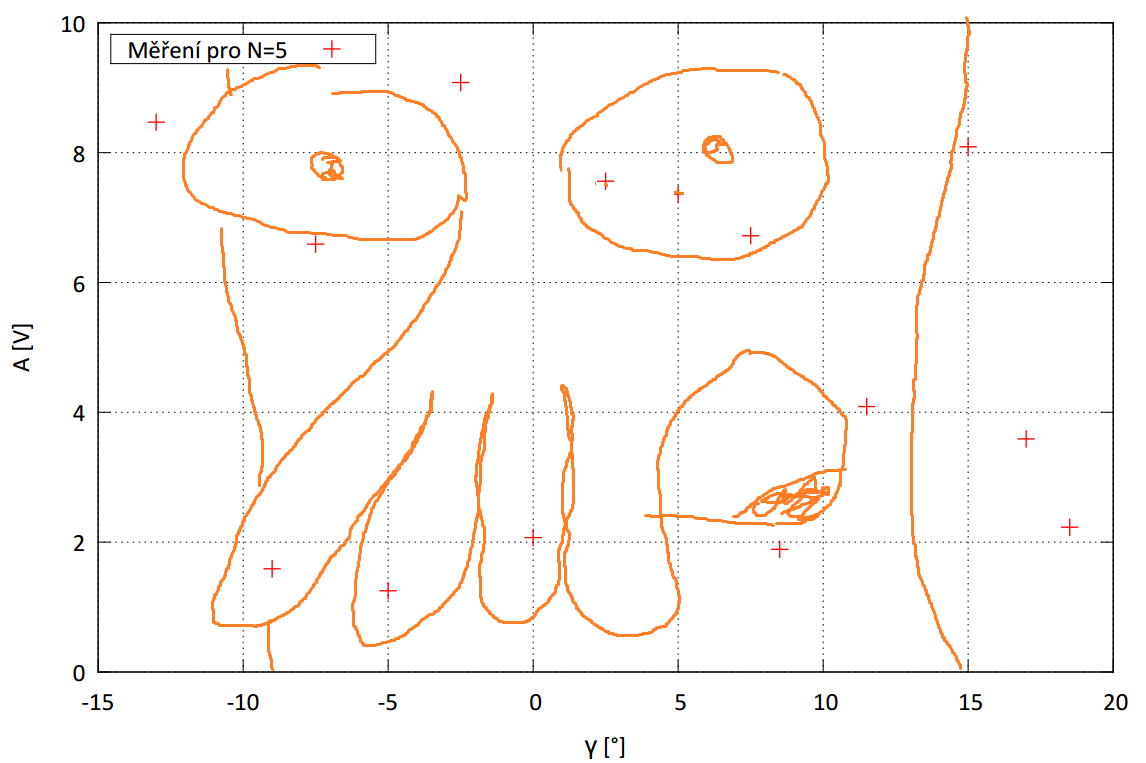
\includegraphics[width=\linewidth]{att/zoidberg.png}
	    \vspace*{-1cm}    
		\caption{Ani funkce \emph{"Why not Zoidberg?"} na naše hodnoty nestačila.}
		\label{fig:g_fun_3}
	\end{center}
	\end{figure}
		
% --- Konec dokumentu --------------------------------------------------


\end{document}

